\documentclass[]{article}
\usepackage{amssymb}
\usepackage{amsmath}
\usepackage[utf8]{inputenc}
\usepackage{graphicx}
\usepackage{booktabs}
\usepackage{listings}
\usepackage{color}
\usepackage{tabularx}
\usepackage{hyperref}

\definecolor{dkgreen}{rgb}{0,0.6,0}
\definecolor{gray}{rgb}{0.5,0.5,0.5}
\definecolor{mauve}{rgb}{0.58,0,0.82}

\lstset{frame=tb,
	%language=C++,
	aboveskip=3mm,
	belowskip=3mm,
	showstringspaces=false,
	columns=flexible,
	basicstyle={\small\ttfamily},
	numbers=none,
	numberstyle=\tiny\color{gray},
	keywordstyle=\color{blue},
	commentstyle=\color{dkgreen},
	stringstyle=\color{mauve},
	breaklines=false,
	breakatwhitespace=true,
	tabsize=2
}

\title{FYS-STK4155 - Project 1}
\author{Olav Fønstelien}

\begin{document}
\maketitle

\begin{abstract}
%The abstract gives the reader a quick overview of what has been done and the most important results. Try to be to the point and state your main findings. It could be structured as follows 
% - Short introduction to topic and why its important 
% - Introduce a challenge or unresolved issue with the topic (that you will try to solve) 
% - What have you done to solve this 
% - Main Results 
% - The implications

\end{abstract}

\section{Introduction}
%When you write the introduction you could focus on the following aspects
% - Motivate the reader, the first part of the introduction gives always a motivation and tries to give the overarching ideas
% - What I have done
% - The structure of the report, how it is organized etc
OLS, Ridge and LASSO are three popular methods for linear regression. They are related to each other in that Ridge and LASSO (least absolute shrinkage and selection operator) are refinements of OLS (ordinary least squares) in that they aim to \textit{shrink} the coefficient estimates $\mathbf{\hat{\beta}} \in \mathbb{R}^p$ towards zero by penalizing their value and hence reducing their variance \cite{james2013introduction}.

In this report we will study each of these methods and how they perform when they are applied on $n$th degree polynomial fit with two variables. First we will do a controlled, qualitative study where we will fit each of them to \textit{Franke}'s function, and look at how they perform when varying the number of samples, the number of features and the method of resampling. Then we will move on to an evaluation of their suitability when approximating a highly irregular data set of unknown quality. For this we will use altitude levels of a mountain range. 

% ADD MORE ABOUT RESULTS AND CONCLUSIONS

\section{Methods}
% - Describe the methods and algorithms
% - You need to explain how you implemented the methods and also say something about the structure of your algorithm and present some parts of your code
% - You should plug in some calculations to demonstrate your code, such as selected runs used to validate and verify your results. The latter is extremely important!! A reader needs to understand that your code reproduces selected benchmarks and reproduces previous results, either numerical and/or well-known closed form expressions.

Given a data set $\mathcal{L} = \{(y_i, \mathbf{x}_i), i=0,1,...,n-1\}$ where $\mathbf{y} = \{y_i\}$ are the response variables and $\mathbf{X} = \{\mathbf{x}_i\}$ are the predictors. Let's assume that the predictor $\mathbf{X}$ in $\mathcal{L}$ only partially explains the response variable $\mathbf{y}$, and that there is some underlying function $\mathbf{f}(\mathbf{X})$ in $\mathbf{y}$, such that $\mathbb{E}(\mathbf{y}) = \mathbf{f}(\mathbf{X})$ and
\begin{equation}
\label{y_f_eps}
\mathbf{y} = \mathbf{f}(\mathbf{X}) + \mathbf{\epsilon} \quad \text{, where} \quad \mathbf{f}(\mathbf{X}) = \mathbf{X} \mathbf{\beta} \quad \text{and} \quad \mathbf{\epsilon} \sim \mathcal{N}(0, \sigma^2).
\end{equation}
In linear regression we aim find the best approximation $\mathbf{\tilde{y}} = \mathbf{X\hat{\beta}}$ to $\mathbf{f}$ by minimizing a cost function $C(\mathbf{X},\mathbb{\beta})$, which reflects the expected test error of the approximation \cite{james2013introduction}.

For OLS, the cost function is simply given by the mean squared error (MSE) of the approximation
\begin{equation}
	C_{OLS}(\mathbf{X},\mathbb{\beta}) = \frac{1}{n} \sum_{i=0}^{n-1} (y_i - \tilde{y}_i)^2.
\end{equation}
Now, given Equation (\ref{y_f_eps}), we split the cost function into
\begin{equation*}
\begin{aligned}
	C_{OLS}(\mathbf{X},\mathbb{\beta}) = \frac{1}{n} \sum_{i=0}^{n-1} (y_i - \tilde{y}_i)^2 &= \mathbb{E}[(\mathbf{y} - \mathbf{\tilde{y}})^2] = \mathbb{E}[(\mathbf{f} + \mathbf{\epsilon} - \mathbf{\tilde{y}})^2] \\
	&= \mathbb{E}[(\mathbf{f} - \mathbf{\tilde{y}})^2 + 2(\mathbf{f} - \mathbf{\tilde{y}})\mathbf{\epsilon} + \mathbb{E}(\mathbf{\epsilon}^2),
\end{aligned}
\end{equation*}
and since $\mathbb{E}(\mathbf{f}) = \mathbb{E}(\mathbf{\tilde{y}})$ we get OLS's cost function on the form \cite{james2013introduction}
\begin{equation}
\label{red-irred}
	C_{OLS}(\mathbf{X},\mathbb{\beta}) = \mathbb{E}[(\mathbf{f} - \mathbf{\tilde{y}})^2] + \sigma^2.
\end{equation}
The first term is the MSE of our approximation $\mathbf{\tilde{y}}$ to $\mathbf{f}$, which we aim to minimize. The second term is dependent on the data quality (instrument precision, round-off error, etc.) and is irreducible, or rather; reduction of the cost function beyond $\sigma^2$ leads to overfitting of the model.

The first term in equation (\ref{red-irred}) can be reduced into model \textit{bias} and model \textit{variance}, as outlined in \cite{friedman2001elements}. An approximation $\mathbf{\tilde{y}} = \mathbf{X\hat{\beta}}$ to $\mathbf{f}$ with too low complexity, say $\mathbf{\hat{\beta}} \in \mathbb{R}^2$, will have low variability in its response to different training sets, but the error will be heavily dependent on the choice of model, which is the bias. A too complex approximation, on the other hand, will have high variability in its test response, but generally be less biased. The first term in equation (\ref{red-irred}) can be reduced further to reflect this:
\begin{equation}
\begin{aligned}
\mathbb{E}[(\mathbf{f} - \mathbf{\tilde{y}})^2] &= \mathbb{E}[[(\mathbf{f} - \mathbb{E}(\mathbf{\tilde{y}})) - (\mathbf{\tilde{y}}- \mathbb{E}(\mathbf{\tilde{y}}))]^2] \\ 
&= \mathbb{E}[(\mathbf{f} - \mathbb{E}(\mathbf{\tilde{y}}))^2] - 2\mathbb{E}[(\mathbf{f} - \mathbb{E}(\mathbf{\tilde{y}}))(\mathbf{\tilde{y}}- \mathbb{E}(\mathbf{\tilde{y}}))] + \mathbb{E}[(\mathbf{\tilde{y}}- \mathbb{E}(\mathbf{\tilde{y}}))^2],
\end{aligned}
\end{equation}
where the second term reduces to zero since $\mathbb{E}[\mathbb{E}(\mathbf{\tilde{y}})] = \mathbb{E}(\mathbf{\tilde{y}})$. The cost function can thus be written on the form
\begin{equation}
\begin{aligned}
\label{bias-variance}
C_{OLS}(\mathbf{X},\mathbb{\beta}) &= \mathbb{E}[(\mathbf{f} - \mathbb{E}(\mathbf{\tilde{y}}))^2] + \mathrm{Var}(\mathbf{\tilde{y}}) + \sigma^2 \\
&=\frac{1}{n}\sum_i(f_i-\mathbb{E}\left[\boldsymbol{\tilde{y}}\right])^2+\frac{1}{n}\sum_i(\tilde{y}_i-\mathbb{E}\left[\boldsymbol{\tilde{y}}\right])^2+\sigma^2,
\end{aligned}
\end{equation}

and hence, to obtain the best possible expected test error we must trade bias off against variance.

For OLS, a better fit may be obtained by increasing model complexity to reduce the bias, up to the point where variance starts to influence the model negatively. To allow increasing complexity further, a larger training data set must be used. Ridge and LASSO, however, allows us to further increase model complexity without increasing the training data, by putting an \textit{extra} cost on variance. Since 
\begin{equation}
	\mathrm{Var}(\mathbf{\tilde{y}}) = \mathbb{E}[[\mathbf{X \hat{\beta}} - \mathbb{E}(\mathbf{X \hat{\beta}})]^2] \sim \mathrm{Var}(\mathbf{\hat{\beta}}),
\end{equation}
reducing $\mathrm{Var}(\mathbf{\hat{\beta}})$ reduces $\mathrm{Var}(\mathbf{\tilde{y}})$. Ridge does this by putting a cost $\sum \lambda \beta_j^2$ on the coefficient values, shrinking larger coefficients more than smaller coefficients, while LASSO puts a cost $\sum \lambda |\beta_j|$ on the values which will try to drive them all the way to zero. See equations (\ref{cost-ridge}) and (\ref{cost-lasso}). Figure \ref{fig:ols-ridge-lasso-comp} below shows a comparison for the simple case $\tilde{y} = \hat{\beta}_0 + \hat{\beta}_1x$.
\begin{equation}
\label{cost-ridge}
C_{Ridge}(\mathbf{X},\mathbb{\beta}) = \mathbb{E}[(\mathbf{y} - \mathbf{\tilde{y}})^2] + \sum_{i=1}^{n} \lambda \beta_j^2
\end{equation}
\begin{equation}
\label{cost-lasso}
C_{LASSO}(\mathbf{X},\mathbb{\beta}) = \mathbb{E}[(\mathbf{y} - \mathbf{\tilde{y}})^2] + \sum_{i=1}^{n} \lambda |\beta_j|
\end{equation}

\begin{figure}[!htb]
	\centering
	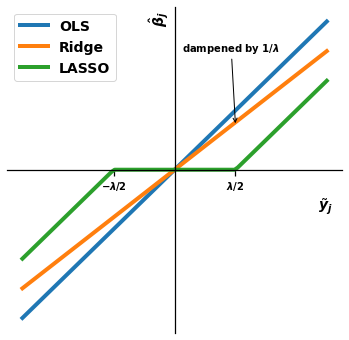
\includegraphics[width=.5\linewidth]{./results/ols-ridge-lasso-comp.png}
	\caption{The effect of shrinking the coefficient estimates in Ridge and LASSO regression methods compared to OLS for the simple approximation $\tilde{y} = \hat{\beta}_0 + \hat{\beta}_1x$. We see that Ridge will try to dampen $\hat{\beta}_1$ to reduce $\tilde{y}$'s variance, while LASSO drives $\hat{\beta}_1$ to zero when it becomes sufficiently small.}
	\label{fig:ols-ridge-lasso-comp}
\end{figure}


\subsection{OLS Regression}
The linear regression model $\mathbf{y} = \mathbf{X\beta} + \mathbf{\epsilon}$ has the closed form solution for the optimum coefficient estimates \cite{van2015lecture}
\begin{equation}
\label{osl-reg}
	\mathbf{\hat{\beta}} = (\mathbf{X}^\intercal \mathbf{X})^{-1} \mathbf{X}^\intercal \mathbf{y},
\end{equation}
which gives us the approximation $\mathbf{\tilde{y}} = \mathbf{X\hat{\beta}}$ to $\mathbf{f}$. We want to approximate the Franke function, given by
\begin{equation}
\begin{aligned}
f(x,y) &= \frac{3}{4}\exp{\left(-\frac{(9x-2)^2}{4} - \frac{(9y-2)^2}{4}\right)}+\frac{3}{4}\exp{\left(-\frac{(9x+1)^2}{49}- \frac{(9y+1)}{10}\right)} \\
&+\frac{1}{2}\exp{\left(-\frac{(9x-7)^2}{4} - \frac{(9y-3)^2}{4}\right)} -\frac{1}{5}\exp{\left(-(9x-4)^2 - (9y-7)^2\right) }.
\end{aligned}
\end{equation}
An $n$th degree polynomial in two variables $p_n(x,y) = 1 + x + y + x^2 + xy + y^2 ...$ can be used to approximate any function in two variables, such as the Franke function. We begin by collecting $m$ samples of the function $\mathcal{L}_{Franke} = \{(f(x_i, y_i), (x_i, y_i), i=0,1,...,m-1\}$. Then we set up our \textit{design matrix} $\mathbf{X}$ by evaluating each of the terms in $p_n(x_i,y_i)$ and installing them in row $i$ of $\mathbf{X}$:
\begin{equation}
\mathbf{x}_i = [1 \quad x_i \quad y_i \quad x_i^2 \quad xy \quad y_i^2 \quad \cdots],
\end{equation}
and install this in equation (\ref{osl-reg}) to get the best MSE fit to the $m$ samples in $\mathcal{L}_{Franke}$. 





\subsection{Ridge Regression}


\subsection{LASSO Regression}


\section{Results}
% - Present your results
% - Give a critical discussion of your work and place it in the correct context.
% - Relate your work to other calculations/studies
% - An eventual reader should be able to reproduce your calculations if she/he wants to do so. All input variables should be properly explained.
% - Make sure that figures and tables should contain enough information in their captions, axis labels etc so that an eventual reader can gain a first impression of your work by studying figures and tables only.



\section{Conclusion}
% - State your main findings and interpretations
% - Try as far as possible to present perspectives for future work
% - Try to discuss the pros and cons of the methods and possible improvements



\bibliographystyle{plain}
\bibliography{project1.bib}
\end{document}
